\documentclass[../main/main.tex]{subfiles}

\newdate{date}{20}{12}{2019}


\begin{document}

\chapter{Renormalization group theory. Universality}

\marginpar{ \textbf{Lecture 20.} \\  \displaydate{date}. \\ Compiled:  \today.}

\section{Renormalization group theory (RG)}

Kadanoff's argument for the Ising model allows us to explain the scaling form of the free energy density and of the correlation length near the critical point; in particular, the Kadanoff's block spin transformation justifies the Widom scaling hypothesis and identifies \( \lambda  \) with \( l \). We have obtained the results:
\begin{equation*}
  \begin{cases}
   f_s (t,h) = l^{-d} f_s \qty(t l^{y_t}, h l^{y_h}) \\
   G (\va{r},t,h) = l^{-2(d-y_h)} G \qty(\frac{\va{r}}{l}, t l^{y_t}, h l^{y_h}) \\
   t_l = t l ^{y_t}, \quad h_l = h^{y_h}
  \end{cases}
\end{equation*}
where we did two crucial assumptions:
\begin{enumerate}
\item \( 1^{st} \) assumption:
 \begin{equation*}
  \mathcal{H}_l = \mathcal{H}_\Omega
\end{equation*}
\item \( 2^{nd} \) assumption:
\begin{equation*}
  \begin{cases}
   t_l = t l^{y_t}\\
   h_l = h l^{y_h}
  \end{cases}
\end{equation*}
\end{enumerate}
 \noindent However, as we have seen, the Kadanoff's theory is unable to predict the values of the scaling exponents \( y_t \) and \( y_h \)  (and thus ultimately of the critical exponents), nor can it explain why universality occurs.

 \begin{remark}
 Open problems are: how an iterative procedure of coarse-graining can produce the \( 2^{nd} \) assumption? How this can gives rise to the singular behaviour of \( f_s \)? How can we explain universality of the critical points?
 \end{remark}


We will see that these problems are solved with the introduction of the Renormalization Group (done by K. G. Wilson at the beginning of the '70s), which we will call simply "RG" from now on for the sake of simplicity. The RG is based upon the correct "intuition" of Kadanoff's argument that the coupling constants of a Hamiltonian change if we coarse-grain the system (or in other words we "look" at it on different spatial scales); however, this "intuition" strictly speaking is not correct since we have seen that in Kadanoff's procedure we assume that after the coarse-graining procedure the Hamiltonian of the system has exactly the same form: as we will see, this is not true in general because new terms can appear after we coarse-grain the system.

\subsection{Main goals of RG}
The main goals of the Renormalization Group theory are:
\begin{enumerate}
\item To fornish an algorithm way to perform systematically the coarse graining procedure.

More specifically, the realization of a coarse graining procedure, also called decimation, is like the one introduced by Kadanoff for the Ising model; in general, this procedure must integrate the degrees of freedom of the system on scales of linear dimension \( la \)  which must be much larger than the characteristic microscopic scale \( a \) of the system, but also much smaller than the correlation length \( \xi  \):
\begin{equation*}
  a \ll la \ll \xi
\end{equation*}
 After the decimation, we are left with a new effective Hamiltonian that describes the system at larger length scales. We will see that this is equivalent to find a transformation between the coupling constants \( K \rightarrow K' \).

\item Identify the origin of the critical behaviour and explain universality.

The coarse graining procedure will give rise to a system with \( \xi_l = \xi /l \),
this means that the new correlation length is smaller than the original one, so our system is farther from criticality after the decimation.

\end{enumerate}

To make an example, suppose we are given a generic Hamiltonian \( \mathcal{H} = \mathcal{H} ([K]) \) which depends on an arbitrary number of coupling constants
\( [K] = \va{K} = \qty(K_1,K_2,\dots K_n)  \) (in the case of an Ising model with nearest-neighbour interaction and an external field there are only two coupling constants, \( K = K_1 \) and \( h = K_2 \)).

Let us suppose we apply a coarse-graining procedure, in which we integrate the degree of freedom within distance \( l \) with \( a \le la \le L \).
For what we have just stated, the action of the RG can be expressed as a transformation of the coupling constants:
\begin{empheq}[box=\myyellowbox]{equation}
  [K'] = \mathcal{R}_l [K], \quad l > 1
  \label{eq:20_1}
\end{empheq}
where \( \mathcal{R}_l \) is called \emph{RG transformation},  while this last equation is referred to as \emph{recursive relation}.


\subsubsection{Properties of \( \pmb{\mathcal{R}_l} \)}

We suppose that the function \( \mathcal{R}_l \) satisfy the following properties:

\begin{enumerate}
\item \( \mathcal{R}_l \) is \textbf{analytic} (sum of a finite number of degrees of freedom, no matter how complicated it may be).


\item The set of  transformations \( \mathcal{R}_l \) forms a \textbf{semigroup}, because if we subsequently apply two transformations \(\mathcal{R}_{l_1}  \) and \(\mathcal{R}_{l_2}  \) on two different length scales \( l_1 \)  and \( l_2 \) we have:
\begin{equation*}
  \begin{cases}
   [K'] = \mathcal{R}_{l_1} [K] \\
  [K''] = \mathcal{R}_{l_2} [K'] = \mathcal{R}_{l_2} \circ \mathcal{R}_{l_1} [K]
  \end{cases}
\end{equation*}
Hence, we have the relation
\begin{equation}
  \mathcal{R}_{l_2 l_1} [K] = \mathcal{R}_{l_2} \circ \mathcal{R}_{l_1} [K]
\end{equation}

\begin{remark}
Note that it is a \emph{semigroup} and not a \emph{group}, since in general does not exist the inverse transformation; in fact, we should have always \( l>1 \).
\end{remark}

There is no general way to construct the function \(  \mathcal{R}_l  \): depending on the system and on the case considered we can choose different ways to carry out the decimation, and in general (as we will see) for a given system many different RG transformations can be built. In general such procedures can be done either in coordinate space (real space Renormalization Group) or in Fourier space (momentum shell Renormalization Group).

In terms of the coupling constants \( [K] \) the partition function of the original system is:
\begin{equation*}
  Z_N [K] = \Tr e^{-\beta \mathcal{H}[K]}
\end{equation*}
while the free energy density is
 \begin{equation*}
   f_N [K] = - \frac{k_B T}{N} \log{Z_N [K]}
 \end{equation*}

 Now, if the RG transformation integrates the degrees of freedom on the spatial scale \( la \)  then the number of degrees of freedom will decrease by a factor \( l^d \), if \( d \) is the dimensionality of the system; in other words, after the RG transformation \( \mathcal{R}_l \), the number \( N \) of degrees of freedom is reduced by
\begin{equation*}
  N_l = \frac{N}{l^d}
\end{equation*}

\item The new hamiltonian \( \mathcal{H}_l [K'] \) can be (and in general it is) different from the previous one \( \mathcal{H} [K] \) (this is the main difference with the Kadanoff's theory), but the effective Hamiltonian \(  \mathcal{H}_l [K']\)  must have the same symmetry properties of the original one!

This means (and this is the great improvement with respect to Kadanoff's argument) that the decimation can make some new terms appear in the coarse-grained Hamiltonian, as long as they respect the same symmetries of the original system. In other words, if \( K_m=0 \)  in \( \mathcal{H}_N \)  but its relative term is allowed by the symmetry group of \( \mathcal{H}_N \)  itself, then we can have \( K_m' \neq 0 \) in \( \mathcal{H}_{N'}' \).

For example, if we start from
\begin{equation*}
  \mathcal{H}_N = N K_0 + K_2 \sum_{ij}^{} S_i S_j
\end{equation*}
if the term \( K_3 \) is not allowed by the symmetry group of \( \mathcal{H}_N \), we cannot produce
\begin{equation*}
  \mathcal{H}_{N'}' = N' K_0' + K_1' \sum_{I}^{} S_I + K_2' \sum_{IJ}^{} S_I S_J
  + \mathcolorbox{red!20}{ K_3' \sum_{IJK}^{} S_I S_J S_K}
\end{equation*}

\item The invariance condition is not in \( \mathcal{H} \) (as in Kadanoff's theory) but in \( Z \); hence, the coarse-graining procedure (decimation) leaves invariant the partition function instead of the Hamiltonian:
\begin{equation}
  Z_{N'} [K'] = Z_N [K]
  \label{eq:20_2}
\end{equation}
this invariance condition has a consequence on the free-energy:
  \begin{equation*}
  f_N [K]  \simeq \frac{1}{N} \log{Z_N [K]} \simeq \frac{l^d}{l^d N} \log{Z_{N'}[K']} \simeq l^{-d} \frac{1}{N'} \log{Z_{N'}} [K']
\end{equation*}
where \( N' = N/l^d \).
Hence,
\begin{equation}
  f [K] \propto l^{-d} f [K']
\end{equation}
which is the scaling form of the free energy density as obtained by Kadanoff.

\end{enumerate}



\subsection{Singular behaviour in RG}

We have stated that the RG transformations \( \mathcal{R}_l \) are analytic, hence a single \( \mathcal{R}_l \) involves the integration of a finite number of dregrees of freedom and the free energy cannot develop the singularity behaviour we are looking for; so, we might ask: where does the singular behaviour of a system near a critical point come from? This occurs in the thermodynamic limit, which in this case is obtained when we apply the RG transformation an infinite number of times. Indeed, in order to integrate a thermodynamic number of degrees of freedoms, one has to apply an infinite number of RG transformations.

In general, after the \( n \)-th iteration of the RG, the coarse-graining length of the system will be \( l \rightarrow l^n \) and the coupling constants \( [K] \rightarrow [K^{(n)}] \).
As \( n \) increases the "vector" of coupling constants describes a "trajectory" in the space of all the possible coupling constants \( [K] \), often called \emph{Hamiltonian space}, or theory space;
by varying the initial conditions, namely different initial Hamiltonians, one obtains a
\emph{flux of trajectories} (i.e. the set of all the trajectories that start from different initial conditions).
In general, these trajectories can form strange attractors or complex limit cycles; however, it is almost always found that they are simply attracted towards or ejected from \emph{fixed points} (cases where this doesn't occur are really exotic), so in the following we will assume that the flux of trajectories only exhibits fixed points.

The study of the properties of the flux of trajectories near these fixed points is crucial, since as we will see it is that that will allow us to actually explain universality and predict the values of the critical exponents (the scaling behaviour introduced by Widom is related to the behaviour of the trajectories close to some fixed points). We therefore proceed to study such points.



 \subsection{Zoology of the fixed points}
 A fixed point \( k^* \) of \( \mathcal{R}_l [k] \) satisfies
 \begin{equation}
   [k^*] = \mathcal{R}_l [k^*]
 \end{equation}
On the other hand, we know that
\begin{equation}
  \xi [k'] = \frac{\xi [k]}{l} \equiv \xi _l
 \end{equation}
At the fixed point
\begin{equation}
  \xi [k^*] = \frac{\xi [k^*]}{l}
\end{equation}
There are two cases:
\begin{equation}
  \xi [k^*] =
  \begin{cases}
   0 & \text{trivial}\\
   \infty & \text{critical}
  \end{cases}
\end{equation}
Each fixed point has its own basin of attraction. This is defined as the set \( \{ [k] \}   \) such that
\begin{equation}
  \mathcal{R}_l^{(n)} [k] \overset{n \rightarrow \infty }{\longrightarrow} [k^*]
\end{equation}
\begin{theorem}{}{}
All the points \([k]  \) belonging to a basin of attraction of a critical fixed point have their correlation length \( \xi = \infty  \).
\end{theorem}
\begin{proof}
\begin{equation}
  \xi [k] = l \xi [k^{(1)}] = \dots l^n \xi [ k^{(n)}]
\end{equation}
If \( [k] \) is in basin of attraction of \( [k^*] \), we have
\begin{equation}
  [k^{(n)}] \overset{n \rightarrow \infty }{\longrightarrow} [k^*]
\end{equation}
On the other hand, \( \xi [k^*] = \infty  \), so
\begin{equation}
  \Rightarrow \xi [k] = l^n \xi [k^*] = \infty
\end{equation}
\end{proof}
\begin{definition}{Critical manifold}{}
 Set of \( [k] \) that forms the basin of attraction of a critical fixed point.
\end{definition}

\subsubsection{Universality}
All the critical models that belong to the critical manifold, have the same critical behaviour of the corresponding critical fixed point. Study the behaviour of \( \mathcal{R}_l \) close to the fixed points.

\subsection{Linearization of RG close to the fixed points and critical exponents}
Let \( [k^*] \) be a fixed point of \( \mathcal{R}_l \) and consider
\begin{equation}
  \va{k} = \va{k}^* + \delta \va{k}
\end{equation}
In components, the RG transformation is
\begin{equation}
  k'_j = (\mathcal{R}_l)_j (\va{k}^*+ \delta \va{k} )
= k^*_j + \sum_{i}^{} \qty(\pdv{k_j'}{k_i} )_{\va{k}^*} \delta k_i + O \qty(\delta k_i^2)
\end{equation}
The linearized transformation is
\begin{equation}
  \delta \va{k}' = \bar{\pi } \delta \va{k}
\end{equation}
where
\begin{equation}
  \qty(\bar{\pi } )_{ij} = \qty(\pdv{k_j'}{k_i} )_{\va{k}^*}
\end{equation}
is a square matrix
\begin{enumerate}
\item \( \bar{\pi }  \) is in general not symmetric. One has to distinguish between left and right eigenvectors.
\item \( \bar{\pi }  \) is not always diagonalizible or sometimes the eigenvalues are complete. For most of the physical system, however, \( \bar{\pi }  \) can be diagonalized and the eigenvalues are real.
\end{enumerate}
Let \( \lambda _l^{(\sigma)} \) be the \( \sigma  \)-esim eigenvalue and \( \va{l}^{(\sigma )} \) the corresponding eigenvector
\begin{equation}
  \Rightarrow \bar{\pi }^{(l)}_{ij} l^{(\sigma )}_j = \lambda _l^{(\sigma )} l_i ^{(\sigma )}
\end{equation}
this is the eigenvalue equation.
Since the \( \mathcal{R}_l \)'s form a semi-group
\begin{equation}
  \bar{\pi }^{(l)} \bar{\pi }^{(l')} = \bar{\pi }^{(ll')}
\end{equation}
and
\begin{equation}
  \lambda _l^{(\sigma )} \lambda _{l'}^{(\sigma )} =  \lambda _{ll'}^{(\sigma )}
  \label{eq:20_3}
\end{equation}
By solving \eqref{eq:20_3} one can show
\begin{equation}
   \lambda _{l}^{(\sigma )} = l^{(Y_\sigma)}
\end{equation}
where \( Y_\sigma \) is the critical exponent to be determined.

How \( \delta \va{k} \) behaves under the linearized transformation \( \bar{\pi }  \)?

Let us expand \( \delta \va{k} \) in terms of \( \va{l}^{(\sigma )} \) (that is a complete orthonormal base)
\begin{equation}
  \delta \va{k} = \sum_{\sigma }^{} a^{(\sigma )} \va{l}^{(\sigma )}
\end{equation}
where
\begin{equation}
  a^{(\sigma )} = \va{l}^{(\sigma )} \vdot \delta \va{k}
\end{equation}
\begin{remark}
Ortonormality is not always true since in general \( \bar{\pi }  \) is not symmetric!
\begin{equation}
  \delta \va{k}' = \bar{\pi } \delta \va{k} = \sum_{\sigma }^{} a^{(\sigma )} \bar{\pi } \qty(\va{l}^{(\sigma )})
  = \sum_{\sigma }^{} a^{(\sigma )} \lambda ^{(\sigma )} \va{l}^{(\sigma )}
  = \sum_{\sigma }^{} a^{(\sigma )'} \va{l}^{(\sigma )}
\end{equation}
where \( a^{(\sigma )'} \) is the projection of \( \delta \va{k}' \) on \( \va{l}^{(\sigma )} \).
  \end{remark}
Same components of \( \delta \va{k} \) grow under the action of \( \bar{\pi }  \) while same others shrink.
If we order the eigenvalues in descending order
\begin{equation}
  \abs{\va{\lambda }_1} \ge \abs{\va{\lambda }_2} \ge \abs{\va{\lambda }_3} \ge \dots \abs{\va{\lambda }_{\sigma}}
\end{equation}
threee cases can occur
\begin{enumerate}
\item Case \( \abs{\lambda ^{(\sigma )}} > 1 \) (i.e. \( y^\sigma > 0\)): implies that \( a^{(\sigma )} \) grows under \( \bar{\pi }  \). There are relevant eigenvalues/eigenvectors.

\item Case \( \abs{\lambda ^{(\sigma )}} < 1 \) (i.e. \( y^\sigma < 0\)): implies that \( a^{(\sigma )} \) decreases under \( \bar{\pi }  \). There are irrelevant eigenvalues/eigenvectors.

\item Case \( \abs{\lambda ^{(\sigma )}} = 1 \) (i.e. \( y^\sigma =  0\)): implies that \( a^{(\sigma )} \) remains constant under \( \bar{\pi }  \). There are marginal eigenvalues/eigenvectors.
\end{enumerate}

Starting from a point close to a critical fixed point \( \va{k}^* \) (but not on the critical manifold), the trajectory will abandau \( [k^*] \) along the relevant directions whereas it will approach \( [k^*] \) along the irrelevant directions.

\begin{itemize}
\item \emph{Irrelevant eigenvectors} form the local basis of the basin of attraction of \( [k^*] \).
\item \emph{Relevant eigenvectors} codimension \( C \) of the basin of attraction.
\end{itemize}
\begin{remark}
The eigenvalues and the corresponding eigenvectors depend on the chosen fixed point \( [k^*] \).
\end{remark}

\section{RG and scaling}
Let
\begin{equation}
  \begin{cases}
   k_1 \rightarrow k_1 (T) = T\\
   k_2 \rightarrow k_2 (H) = H
  \end{cases}
\end{equation}
for simplicity. Suppose to perform a RG transformation \( \mathcal{R}_l \) such that
\begin{equation}
  \begin{cases}
   T' = \mathcal{R}_l ^T (T,H) \\
   H' = \mathcal{R}_l ^H (T,H)
  \end{cases}
\end{equation}
The critical fixed point is defined as
\begin{equation}
  \begin{cases}
   T^* = \mathcal{R}_l ^T (T^*,H^*)\\
   H^* = \mathcal{R}_l ^H (T^*,H^*)
  \end{cases}
\end{equation}
with \( \xi (T^*,H^*) = \infty  \).
\begin{remark}
Remember that \( \va{k}^* \equiv (T^*,H^*) \).
\end{remark}
For standard magnetic systems \( H^*=0 \). By linearising around the fixed point
\( \delta \va{k}= (t,h) \)  where
\begin{equation}
  \begin{cases}
   t = \frac{(T-T^*)}{T^*}\\
   h = \frac{(H-H^*)}{H^*}
  \end{cases}
\end{equation}
we obtain
\begin{equation}
  \begin{pmatrix}
  t' \\
  h'
  \end{pmatrix}
  = \bar{\pi }
  \begin{pmatrix}
  t \\
  h
  \end{pmatrix}
\end{equation}
with
\begin{equation}
  \bar{\pi } =
  \begin{pmatrix}
     \pdv{\mathcal{R}_l^T}{T} & \pdv{\mathcal{R}_l^T}{H} \\
     \pdv{\mathcal{R}_l^H}{T} & \pdv{\mathcal{R}_l^H}{H}
  \end{pmatrix}_{T^*,H^*}
\end{equation}
In general the eigenvectors \( \va{l}^{(\sigma )} \) are linear combinations of \( t \) and \( h \). When \( \bar{\pi }  \) can be diagonalized, \( t \) and \( h \) are not mixed. Suppose this is the case and let
\begin{equation}
  \lambda _l ^{(t)} = l^{Y_t}, \quad \lambda _l^{(h)} = l ^{Y_h}
\end{equation}
A linear transformation is
\begin{equation}
  \begin{pmatrix}
  t' \\
  h'
  \end{pmatrix}
  =
  \begin{pmatrix}
  \lambda _l^{(t)}   & 0 \\
    0 & \lambda _l^{(h)}
  \end{pmatrix}
  \begin{pmatrix}
  t \\
  h
  \end{pmatrix}
\end{equation}
After \( n \) iterations, we have
\begin{equation}
  \begin{cases}
   t^{(n)} = \qty(l^{Y_t})^n t  \\
  h^{(n)} = \qty(l^{Y_h})^n h
  \end{cases}
\end{equation}
On the other hand,
\begin{equation}
  \xi ' \equiv \xi (t',h') = \frac{\xi (t,h)}{l}
\end{equation}
and, hence, after \( n \) iterations
\begin{equation}
  \xi (t,h) = l^n \xi \qty(l^{n Y_t} t, l^{n Y_h} h)
\end{equation}
Idea (lesson): we are very close to the critical point (infinite) and we want to go a little bit away in order to not to be anymore infinite. In such a way after \emph{n} iterations we obtain the previous result.
Let \( h=0 \) \( (H=H^*) \), hence
\begin{equation}
  \xi (t,0) = l^n \xi \qty(l^{n Y_t} t , 0)
\end{equation}
Since \( l \) is arbitrary, we can choose it such that
\begin{equation}
  t l ^{n Y_t} = b \gg 1, \quad b \in \R^+
\end{equation}
In such a way we go away from the critical point!
\begin{remark}
\( l \) is not an integer any more.
\end{remark}
\begin{equation}
  \Rightarrow l^n = \qty(\frac{b}{t})^{1/Y_t}
\end{equation}
so, for \( t \rightarrow 0 \)
\begin{equation}
  \xi (t) = \qty(\frac{t}{b})^{-1/Y_t} \xi (b)
\end{equation}
On the other hand, \( \xi \sim t^{-\nu } \), \( t \rightarrow 0 \)
\begin{equation}
  \Rightarrow \nu = \frac{1}{Y_t}
\end{equation}
where
\begin{equation}
  Y_t  = \frac{1}{l} \ln{\lambda _l^t}
  \label{eq:20_4}
\end{equation}
The equation \eqref{eq:20_4} is an important result since it gives a recipe, based on \( \mathcal{R}_l \), to compute \( Y_t \) explicitely!

Similarly,
\begin{equation}
\begin{split}
f_s (t,h)  &= l^{-D} f_s (t',h') = l^{-nD} f_s (t^{(n)},h^{(n)}) \\
& = l^{-nD} f_s \qty(l^{n Y_t}t, l^{n Y_h}h)
\end{split}
\end{equation}
Hence, we get the free energy of the original system, by using the renormalization group!

Let \( l \) such that \( l^{n Y_t} t= b \gg 1\), hence
\begin{equation}
  l^n = \qty(\frac{b}{t})^{1/Y_t}
\end{equation}
\begin{equation}
  f_s (t,h) = t^{D/Y_t} b^{-D/Y_t} f_s \qty(b, \frac{b^{Y_h/Y_t}h}{t^{Y_h/Y_t}})
\end{equation}
that is of the form
\begin{equation}
  f_s (t,h) = \bar{b} t^{2- \alpha } f_s \qty(b, \frac{\bar{b} h}{t^{\Delta }})
\end{equation}
with
\begin{equation}
  \begin{cases}
   2 - \alpha = D \nu = \frac{D}{Y_t}\\
   \Delta = \frac{Y_h}{Y_t}
  \end{cases}
\end{equation}
where \( Y_h \) and \( Y_t \) can be computed as
\begin{equation}
  Y_h = \frac{1}{l} \log{\lambda _l^{(h)}}
\end{equation}
Hence, we have all we need for the computation!

\section{Real space renormalization group on 1D Ising model \( (H=0) \)}
\subsection{Decimation procedure for \( D=1 \)}
Decimation means summing up over all spins.
\( D=1 \) the procedure is clearly exact. Idea: pass from a \( N- \) spins system to one with \( \frac{N}{b} \) spins by summing the remaining \( N- \frac{N}{b} \) spins.


Case b=3 (see Figure \ref{fig:20_1}).

\begin{figure}[h!]
\centering
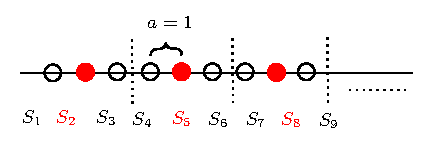
\includegraphics[width=0.6\textwidth]{../lessons/20_image/1.pdf}
\caption{\label{fig:20_1} Description.}
\end{figure}

Sum over the spins with the empty circle at the border of each clok, keeping the spins full circle untouched.
We obtain Figure \ref{fig:20_2}.

\begin{figure}[h!]
\centering
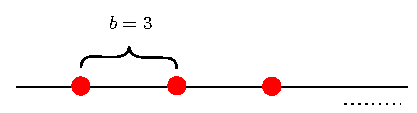
\includegraphics[width=0.6\textwidth]{../lessons/20_image/2.pdf}
\caption{\label{fig:20_2} Description.}
\end{figure}

Let us see how it works for the two blocks \( [S_1,S_2,S_3] \) and \( [S_4,S_5,S_6] \). Let us call
\begin{equation}
  S_2 \equiv S_1', \quad S_5 = S_2' \quad \text{fixed}
\end{equation}
\begin{equation}
  \sum_{S_3 = \pm 1}^{}   \sum_{S_4 = \pm 1}^{}  \exp [ k S_1' S_3 + k S_3 S_4 + k S_4 S_2']
\end{equation}
Since
\begin{equation}
  e^{k S_3 S_4}  = \cosh (k) ( 1 + x S_3 S_4)
\end{equation}
with
\begin{equation}
  x \equiv \tanh k
\end{equation}
we have
\begin{equation}
  \sum_{S_3,S_4}^{} \qty(\cosh k)^3 \qty(1 + x S_1' S_3) \qty(1 + x S_3 S_4) \qty(1 + x S_4 S_2')
\end{equation}
Performing the expansion and summing over \( S_3, S_4 \)  it is easy to show that (to do)
\begin{equation}
  Z_{N'}' (k') = \Tr_{ \{ S_I' \}  } \qty[ 2 ^{2N'} \qty( \cosh k)^{3N'} \qty(1 + x^3 S_I' S_{I+1} )  ]
  \label{eq:20_5}
\end{equation}
This must have the same form of \( Z_N (k) \). Hence, we should rewrite equation \eqref{eq:20_5} as
\begin{equation}
  Z_{N'}' (k') = \Tr_{ \{ S_I' \}  } \exp [ - \beta \mathcal{H}' (k')]
\end{equation}
with
\begin{equation}
  - \beta \mathcal{H}' = N' g (k,k') + k' \sum_{I}^{} S_I' S_{I+1}'
\end{equation}
We note that
\begin{equation}
\begin{split}
2^2 \qty(\cosh k)^3 (1 + x^3 S_I' S_{I+1}')   &=  2^2 \frac{\cosh k'}{\cosh k'}
 \qty(\cosh k)^3  (1 + x^3 S_I' S_{I+1}') \\
 & = 2^2 \frac{(\cosh k)^3}{\cosh k'}
  \qty(\cosh k')  (1 + x' S_I' S_{I+1}') \\
  & = 2^2 \frac{(\cosh k)^3}{\cosh k'}
   \exp (k' S_I' S_{I+1}') \\
   & = \exp [ 2 \ln{2} + \ln{ \qty[ \frac{(\cosh k)^3}{\cosh k'}] }  + k' S_I' S_{I+1}' ]
\end{split}
\end{equation}
It is ok with
\begin{equation}
  \begin{cases}
   g(k,k') = 2 \ln{2} +  \ln{ \qty[ \frac{(\cosh k)^3}{\cosh k'}] } \\
   x' = x^3  \iff k'= \tanh^{-1} \qty[ (\tanh k)^3] \Rightarrow k' = R_{b=3} (k)\\
   N' = \frac{N}{b}
  \end{cases}
\end{equation}
For \( x' = x^3 \), we have two fixed points
\begin{equation}
  \begin{cases}
   x^* = 0 \iff k \rightarrow 0 \iff T \rightarrow \infty \\
   x^* = 1^- \iff k \rightarrow \infty  \iff T \rightarrow 0
  \end{cases}
\end{equation}
For \( \forall x_0 < 1 \), we have \( R^{(n)} \overset{n \rightarrow \infty }{\longrightarrow} 0^+ \), \( x=1 \) is an unstable fixed point, as shown in Figure  \ref{fig:20_3}.
\begin{figure}[h!]
\centering
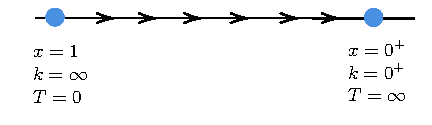
\includegraphics[width=0.6\textwidth]{../lessons/20_image/3.pdf}
\caption{\label{fig:20_3} Description.}
\end{figure}
We have
\begin{equation}
  \xi (x') = \frac{\xi (x)}{b}, \quad \text{with } x' = x^b
\end{equation}
where \( b \) is arbitrary. Let us choose \( b = c / \ln{x}  \):
\begin{equation}
  \xi (x^b) = \xi  \qty(e ^{b \ln{x} }) = \xi (e^c) = \frac{\xi (x)}{b}
  = \qty(\frac{c}{\ln{x} })^{-1} \xi (x)
\end{equation}
Finally,
\begin{equation}
  \xi (e^c) = \frac{\ln{x} }{c} \xi (x) \quad \Rightarrow \xi (x) = \frac{c \xi (e^c)}{\ln{x} } = \frac{const}{\ln{x} }
\end{equation}
\begin{equation}
  \xi (k) = \frac{const}{\ln{\qty(\tanh k) } }
\end{equation}
equal to the exact model in \( D=1 \).
\( k \rightarrow \infty  \) \( (x \rightarrow 1) \), we have
\begin{equation}
  \xi \sim e^{const/T}
\end{equation}
finite \( \forall k \neq \infty  \).

\subsection{Decimation procedure for \( D>1 \) (proliferation of interactions)}
Ioing on a square lattice, block transformation (length \( b \)). There are problems with the spins at the boundaries.
In order to get \( Z_{N'}' (k') = Z_N (k) \), at least an additional term in the Hamiltonian must be introduced
\begin{equation}
  \mathcal{H} \rightarrow \mathcal{H}' = \mathcal{H}' (k',k_2')
\end{equation}
This unfortunately occurs at each iteration! There is an uncontrolled proliferation and approximations are necessary.
\begin{example}{Decimation of Ising on square lattice}{}
  \( x \): spin to sum over
\begin{equation}
  \begin{cases}
   k' = \frac{1}{4} \ln{\cosh 4 k} \\
   L' = \frac{1}{8} \ln{\cosh 4 k} \\
   Q' = \frac{1}{8} \ln{\cosh 4 k} - \frac{1}{2} \ln{\cosh 2 k}\\
  \end{cases}
\end{equation}
(4 spins). The approximations are:
\begin{enumerate}
\item Neglect \( Q' \) term.
\item Omit explicit dependence on \( L' \). Hence, assuming \( k'+L' \rightarrow k' \). 1 recursion
\begin{equation}
  k' = \frac{3}{8} \ln{\cosh 4 k}
\end{equation}
\begin{equation}
  \begin{cases}
   k^{(n)} \overset{n \rightarrow \infty }{\longrightarrow} \infty  & k_0 > k_c \\
   k^{(n)} \overset{n \rightarrow \infty }{\longrightarrow} 0  & k_0 < k_c
  \end{cases}
\end{equation}
where \( \infty ,0 \) are stable fixed point.
\begin{equation}
  \delta k' = \lambda _t \delta k = l^{Y _t} \delta k
\end{equation}
where
\begin{equation}
  \lambda _t = \eval{\dv{k'}{k} }_{k=k_c}
\end{equation}
For \( l = \sqrt{2}  \),
\begin{equation}
\begin{split}
Y_t  &= \frac{\ln{\lambda _t} }{\ln{l} } = \frac{1}{\ln{\sqrt{2} } } \ln{\qty(\dv{k'}{k})_{k=k_c} }   \\
& = \frac{1}{\ln{\sqrt{2} } }  \ln{\qty(\dv{}{k} \qty(\frac{3}{8} \ln{(\cosh 4k)} ) ) } = 1.070
\end{split}
\end{equation}
so, this is actual a relevant eigenvalue.
We have also the critical exponents
\begin{equation}
  \nu = \frac{1}{Y_t} = 0.9345, \quad \alpha = 2 - \frac{d}{Y_t} = 0.1313
\end{equation}
\end{enumerate}

\end{example}








\end{document}
